\documentclass[14pt,a4paper]{extarticle}
\newcommand{\judul}{Besaran, Vektor, Gerak Lurus}
\newcommand{\penulis}{bintangpelajar.com}
\usepackage[latin1]{inputenc}
\usepackage{amsmath}
\usepackage{microtype}
\usepackage[none]{hyphenat}
\usepackage{verbatim}
\usepackage{amsfonts}
\usepackage{amssymb}
\usepackage{enumitem}
\renewcommand{\familydefault}{\sfdefault}
\usepackage{mathpazo}
\renewcommand{\rmdefault}{put}
\usepackage{enumitem}
\usepackage[dvipsnames,svgnames]{xcolor}
\usepackage{tkz-euclide}
\usetkzobj{all}
\usepackage{graphicx}
\usepackage{fancyhdr}
\usepackage{tikz} 	
\usepackage{adjustbox}
\usepackage{multicol}
\usepackage{lipsum}
\usepackage[headsep=0.2cm,footskip=2pt,top=1.2cm,bottom=1cm,left=1cm,right=1cm]{geometry}
\usepackage{cancel} \usepackage{xcolor}
\usepackage{tcolorbox}
\usetikzlibrary{decorations.pathmorphing,patterns}
\usetikzlibrary{decorations.pathreplacing,calc}
\usepackage[framemethod=TikZ]{mdframed}

\newtcolorbox{kotak}{colback=gray!2!white, width=10cm,  before=\par\centering\smallskip, after=\par}
\newtcolorbox{kotakpjg}{colback=gray!2!white, width=18cm, halign=flush center, before=\par\centering\smallskip, after=\par}

\newtcolorbox{contoh}[1] {colback=gray!2!white, colframe=gray!70, fonttitle=\bfseries, title=#1,breakable=true}
\newtcolorbox{kegiatan}[1] {colback=white, colframe=gray!70, fonttitle=\bfseries, title=#1, breakable=true}
\newtcolorbox{catatan}[1][]{%
  enhanced jigsaw, % better frame drawing
  borderline west={2pt}{0pt}{gray}, % straigh vertical line at the left edge
  sharp corners, % No rounded corners
  boxrule=0pt, % no real frame,
  fonttitle={\large\bfseries},
  coltitle={black},  % Black colour for title
  title={ },  % Fixed title
  attach title to upper, % Move the title into the box
  #1
}




 \newcommand\coret[2][red]{\renewcommand\CancelColor{\color{#1}}\cancel{#2}}
\SetLabelAlign{Center}{\hfil\makebox[1.0em]{#1}\hfil}

\newtcolorbox{mybox}[1][] { colframe = blue!10, colback = blue!3,boxsep=0pt,left=0.2em, coltitle = blue!20!black, title = \textbf{jawab}, #1, } 

%---------- kunci (jika 1 ) muncul
\def\tampilkunci{0}
\newcommand{\hide}[1]{\ifnum\tampilkunci=1
%
\begin{mybox}
 #1
\end{mybox}
%
\vspace{\baselineskip}\fi}
\newcommand{\hidebox}[2]{\ifnum\tampilkunci=1
%
 #2
%
\vspace{\baselineskip}\fi\ifnum\tampilkunci=0
%
\vspace{#1cm}\fi}

\newcommand*\kunci[1]{\ifnum\tampilkunci=1
%
\tikz[baseline=(char.base)]{\node[red, shape=circle,draw,inner sep=0.5pt,xshift=2pt](char){#1};}\stepcounter{enumii}
\fi\ifnum\tampilkunci=0
%
\hspace{3pt}#1\stepcounter{enumii}
%
\fi}

%------------- MULAI FUNGSIKU ------------
\newcommand{\cartesius}[3]{
\draw[help lines] (-1,-1) grid (#1);
\foreach \x in {1,2,...,#2}{
\node at (\x,0)[scale=0.5]{\x};}
\foreach \y in {1,2,...,#3}{
\node at (0,\y) [scale=0.5]{\y};}}

\newcommand{\pers}[1]{\begin{align*} #1 \end{align*}}
% \sci{ }  misal  x 10^2  tinggal tulis 
% \sci{2} 
\newcommand{\sci}[1]{$\times 10^{#1}$}

\newcommand{\scip}[1]{\times 10^{#1}}

%----membuat tanda silang di samping text
\newcommand*\silang[1]{\tikz[baseline=(char.base)]{
\draw[red,thick](-0.2,-0.20)--(0.2,0.2);
\draw[red,thick](-0.2,0.20)--(0.2,-0.2);
\node[black](char){#1};
}}
%----- membuat tanda centang di mana saja
\newcommand*\centang[1]{\tikz[baseline=(char.base)]{
\draw[red, very thick](-0.2,0.1)--(-0.1,0)--(0.2,0.3);
\node(char){#1};
}}
%------------mewarnai text merah
\newcommand*\merah[1]{
\textcolor{red}{#1}}
\newcommand*\pilgan[1]{
\begin{enumerate}[label=\Alph*., itemsep=0pt,topsep=0pt,leftmargin=*,align=Center] #1 
\end{enumerate}}

%---- membuat pernyataan pada soal SBMPTN
\newcommand*\pernyataan[1]{
\begin{enumerate}[label=(\arabic*), itemsep=0pt,topsep=0pt,leftmargin=*] #1 
\end{enumerate}}

%------ lebar baris pada tabular
\newcommand{\baris}[1]{\renewcommand\arraystretch{#1} }
%\newcommand{\tabel}[2j]{\begin{tabular}{#1}
%\end{tabular}
\newcommand{\nomortab}[1]{\begin{enumerate}[topsep=0mm,itemsep=0mm,leftmargin=*]#1
\end{enumerate}}
%------------ END OF FUNGSIKU ----------- 





%--------------- begin{document}-----------
\pagestyle{fancy}
\fancyhf{} 
\rhead{\penulis}
\lhead{\judul}
\rfoot{Hal \thepage}
\begin{document}
\begin{tabular}{|p{8cm}|p{9cm}|}
\hline 
\nomortab{\item[1.] Sebutkan besaran-besaran yang termasuk besaran pokok beserta satuannya!} 
& 
\hidebox{10} { ini jawaban} \\ \hline
%------------------------------------------
\nomortab{\item[2.] Tentukan dimensi dari 
\begin{enumerate}[itemsep=0mm,topsep=0mm,leftmargin=*]
\item $P$ daya
\item $E$ Energi
\item $p$ momentum
\end{enumerate}}
& \hidebox{4}{ini jawaban \vspace{10cm} }\\ \hline 
%------------------------------
\nomortab{\item[3.] Tiga gaya $\vec{P}$, $\vec{Q}$, dan $\vec{R}$ membentuk sudut seperti pada gambar di bawah, tentukan berapa resultan ketiga gaya tersebut!

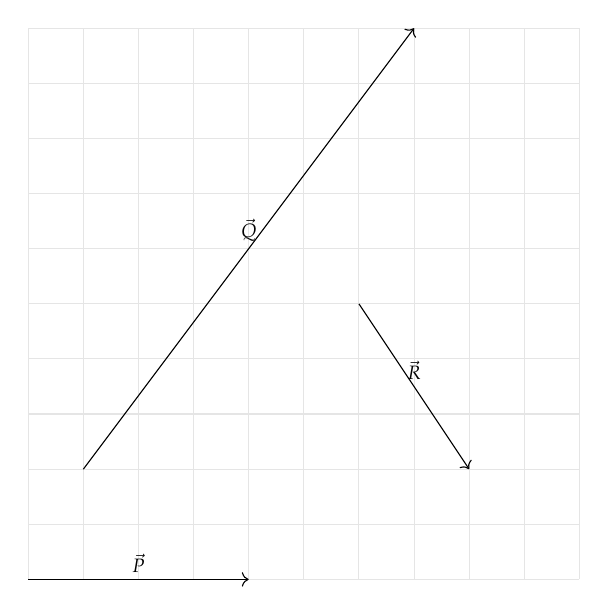
\begin{tikzpicture}[scale=0.7]
\draw[help lines, gray!20](0,0)grid (10,10);
\draw [->] (0,0) --node [above,midway,scale=0.7]{$\vec{P}$}(4,0);
\draw [->] (1,2) -- node [above,midway,scale=0.7]{$\vec{Q}$}(7,10);
\draw [->] (6,5) -- node [above,midway,scale=0.7]{$\vec{R}$}(8,2);
\end{tikzpicture}}
& \hidebox{4}{ini jawaban }\\ \hline 
%------------------------
\nomortab{\item[4.] Tiga vektor $F_1$, $F_2$, dan $F_3$ membentuk gambar seperti pada gambar. Tentukan berapa resultan ketiga gaya tersebut!

\begin{tikzpicture}[scale=0.7]
\draw[<->](0,10)--(0,0)--(10,0);
\draw[<->](-10,0)--(0,0) --(0,-10);
\draw[->](0,0)--(4:60) node [above,scale=0.7]{$\vec{F_1}$};
\draw[->](0,0)--(8.4:135)node [above, left, scale=0.7]{$\vec{F_2}$};
\end{tikzpicture}}
& \hidebox{4}{ini jawaban} \\ \hline




\end{tabular}
%
%------------ nomor 1----------
\begin{enumerate}[itemsep=0mm]

\item Jarum sepanjang 7 cm terapung di permukaan air. Jika massa jarum 1,4 gram, brapa tegangan permukaan air yang mengenai jarum?


%------------ nomor 2 -------------
\item Pembuluh xylem pada tanaman mempunyai jari-jari sekitar 0,01 mm. Jika suhu air 20$^o$, sudut kontak 0$^o$, dan tegangan permukan air 72,8 \sci{-3} N/m. Tentukanlah kenaikan air pada pembuluh xylem akibat adanya kapilaritas! (massa jenis air  = 1000 kg/m$^3$)

%------------- nomor 3 -------------
\item Sebuah logam berbentu bola dijatuhkan ke dalam suatu zat cair kental. Sesuai dengan hukum Stokes maka bola akan mendapatkan gaya gesek ke atas yang besarnya sebagai berikut:
$$ F_s = 6 \pi \eta r v $$
Dimensi koefisien kekentala $\eta$ adalah . . . .

 
%------------ nomo 4 ------------

\item Sebuah bola logam berdiameter 200 mm jtuh ke dalam cairan gliserin yang memiliki viskositas 1,5 Pa.s sehingga memiliki kecepatan 0,2 m/s. Tentukan gaya gesekan Stokes antara bola dan gliserin!

\hide{
untuk itu perlu tahu rumus-rumus pada kekentalan (viskositas) berikut ini.
$$F_s= 6 \pi \eta r v $$
\begin{tabular}{lcl}
$F_s$ &:& Gaya stokes (N) \\
$\eta$ &:& Kekentalan/viskositas (Pa.s)\\
$r$ &:& jari-jari benda "biasanya bola"(m) \\
$v$ &:& kecepatan terminal (m/s) \\
\end{tabular}

Jadi gaya gesek karena benda bergerak di fluida disebabkan oleh adanya kekentalan. Biasa dinamakan Gaya stokes $F_s$ (penemunya). Dipengaruhi oleh empat variabel di atas. Untuk soal ini bisa dijawab dengan mudah.
\pers{
F_s&=6\pi \eta r v \\
F_s&=6\pi (1,5)(2\scip{-1})(0,2)\\
F_s&=36 \pi \scip{-2} \text{N}
} 
}

% ---------------- 
\item Sebuah bola yang massa jenisnya 6,36 gram/cm$^3$ dan diameter 20 mm jatuh ke dalam cairan pelumas yang massa jenisnya 5,10 gram/cm$^3$. Jika kecepatan terminal bola mencapai 0,2 m/s. Tentukan koefisien viskositas cairan pelumas tersebut!
\hide{
Soal ini menggunakan persamaan turunan dari gaya stokes tadi. Namanya persamaan kecepatan terminal. Berikut gambar bola di dalam cairan, ada berat, gaya angkat $F_a$ dan gaya stokes $F_s$

\begin{minipage}[T]{0.2\textwidth}
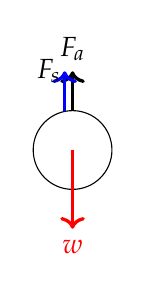
\begin{tikzpicture}
%\cartesius{5,5}{5}{5};
\draw(2,2) circle (0.5);
\draw[->,very thick] (2,2.5) -- (2,3) node [above,scale=1]{$F_a$};
\draw [->, blue, very thick] (1.9,2.5)--(1.9,3);
\node at (1.7,3) {$F_s$};
\draw [->, red,very thick] (2,2) -- (2,1) node [below]{$w$};
\end{tikzpicture}
\end{minipage}
\begin{minipage}[T]{0.6\textwidth}
Jadi agar timbul kecepatan terminal artinya kecepatan konstan ($a$ =0 ) maka jumlah gaya arah vertikal juga harus nol $\Sigma F =0$
\end{minipage}}
\hide{
Menurut hukum Newton dan Stokes, serta gaya angkat archimedes $F_a$ 
\pers{
\Sigma F_y &=0\\
F_a+F_s-w&=0\\
F_a+F_s &= w\\
\rho_f g V_b + 6 \pi \eta r v &= m.g \\
\rho_f g V_b + 6 \pi \eta r v & = \rho_b.V_b.g\\
6 \pi \eta r v & = V_b.g.(\rho_b-\rho_f)\\
v_{t} &= \frac{V_b.g.(\rho_b-\rho_f)}{6 \pi \eta r}\\
}

Padahal benda dimisalkan bola, berarti volumenya adalah $V= \frac{4}{3}\pi r^3$
\pers{
v_t &= \frac{\frac{4}{3}\coret{\pi} r^{\coret{3}^2}.g(\rho_b-\rho_f)}{6 \coret{\pi} \eta \coret{r}}\\
v_t &= \frac{2 g.r^2 (\rho_b-\rho_f)}{9 \eta } 
}
\begin{kotak}
 $$v_t = \frac{2 g.r^2 (\rho_b-\rho_f)}{9 \eta } $$
\end{kotak}
Jadi dihafalkan persamaan terakhir ini. Misalnya untuk menyelesaikan soal ini tinggal masukkan angkanya

\begin{tabular}{ll}
\multicolumn{2}{l}{$\rho_b=6,36$ gram/cm$^3$ = 6360 kg/m$^3$} \\
\multicolumn{2}{l}{$\rho_f=5,10$ gram/cm$^3$ = 5100 kg/m$^3$} \\
$v$ = 0,2 m/s & $d$=20mm\\
\multicolumn{2}{l}{$r$ = 10 mm = 1 \sci{-2} m }

\end{tabular}

Gunakan persamaan tadi,
\pers{
v_t &= \frac{2 g.r^2(\rho_b-\rho_f)}{9 \eta}\\
\eta &= \frac{2g.r^2(\rho_b-\rho_f)}{9 v_t}\\
\eta &=\frac{2.10.(1\scip{-2})^2(6360-5100)}{9(0,2)}\\
\eta &= \frac{10^{-2}1260}{9}=1,40 \text{ Pa.s} 
}
}

\item [6] Sebuah kelereng memiliki massa jenis 0,9 g/cm$^3$ yang memiliki jari-jari 1,5 cm dijatuhkan bebas dalam sebuah tabung yang berisi oli bermassa jenis 0,8 g/cm$^3$ dan koefisien viskositas 0,03 Pa.s. Tentukan kecepatan terminal kelereng tersebut!
\hide{
\begin{tabular}{ll}
\multicolumn{2}{l}{$\rho_b$ = 0,9 g/cm$^3$ = 900 kg/m$^3$ }\\
\multicolumn{2}{l}{$\rho_f$ = 0,8 g/cm$^3$ = 800 kg/m$^3$ }\\
$\eta$ = 0,03 Pa.s & $r$ = 5 \sci{-2} m \\
\end{tabular}
\pers{
v_t &= \frac{2 g.r^2(\rho_b-\rho_f)}{9 \eta}\\
v_t &= \frac{2.10.(5\scip{-2})^2(900-800)}{9(0.03)}\\
v_t &= \frac{5}{0.27} = 18,52 \text {m/s}
}}
 \end{enumerate}
 \end{document}
